\newpage
\section{Die Verklärung Jesu}
\index{Glanz!Jesu}

\textbf{\textit{E(t,e) | Jesus | Spiegelung}}
\index{Externalisierung E(t,e)}
\index{Jesus!Verklärung}
\index{Spiegelung}

\biblerefformat{kurz}
\bibleverse{Mt}(17:1-9)
\begin{BibelSt}
Sechs Tage danach nahm Jesus Petrus, Jakobus und dessen Bruder Johannes beiseite und führte sie auf einen hohen Berg.  Und er wurde vor ihren Augen verwandelt; sein Gesicht leuchtete wie die Sonne und seine Kleider wurden blendend weiß wie das Licht.  Da erschienen plötzlich vor ihren Augen Mose und Elija und redeten mit Jesus.  Und Petrus sagte zu ihm: Herr, es ist gut, dass wir hier sind. Wenn du willst, werde ich hier drei Hütten bauen, eine für dich, eine für Mose und eine für Elija.  Noch während er redete, warf eine leuchtende Wolke ihren Schatten auf sie und aus der Wolke rief eine Stimme: Das ist mein geliebter Sohn, an dem ich Gefallen gefunden habe; auf ihn sollt ihr hören.  Als die Jünger das hörten, bekamen sie große Angst und warfen sich mit dem Gesicht zu Boden.  Da trat Jesus zu ihnen, fasste sie an und sagte: Steht auf, habt keine Angst!  Und als sie aufblickten, sahen sie nur noch Jesus.  Während sie den Berg hinabstiegen, gebot ihnen Jesus: Erzählt niemand von dem, was ihr gesehen habt, bis der Menschensohn von den Toten auferstanden ist.
\end{BibelSt}

\subsection{Impuls}
\begin{impuls}
\begin{figure}
    \centering
    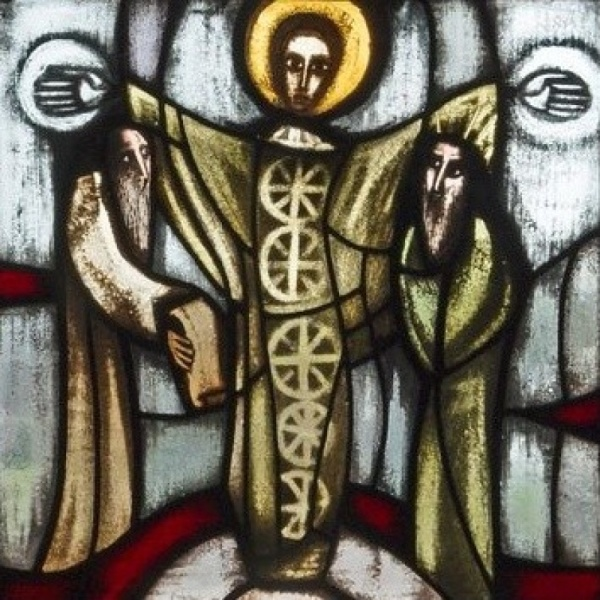
\includegraphics[scale=0.5]
{Pictures/ob_468a26_transfiguration-taize-2.jpg}
    \caption{Transfiguration, Kirche in Taizé}
    \label{fig:Bildmeditation}
\end{figure}

\begin{description}
\item[Petrus, Jakobus und Johannes]Es sind die ersten Jünger, 
\footnote{
\biblerefformat{kurz}
\bibleverse{Lk}(5:1-11); bei 
\biblerefformat{kurz}
\bibleverse{Mk}(4:14-20)
und
\biblerefformat{kurz}
\bibleverse{Mt}(4:18-20) ist auch noch Petrus Bruder Andreas dabei.
}
die Jesus von Anfang an begleitet haben, die auf dem Berg die Verklärung erleben. Bei \biblerefformat{kurz}
\bibleverse{Mt}(26:37) sind es ebenfalls diese drei Jünger, die er später bei seinem Gebet sind Gethsemani noch ein Stück weiter mit sich auf seinem Weg nimmt. Sie erhalten einen Augenblick die Herrlichkeit gezeigt, um sich daran zu erinnern, wenn sie Jesus auf dem Weg durch das Leiden und den Tod bis zur Auferstehung begleitet haben. 
\item[Die Stimme Gottes]«Dass ist mein geliebter Sohn, an dem ich meine Freude habe. Ihm sollt ihr gehorchen.» Die Jünger hören die Stimme Gottes, Jahwes, die ihnen Angst macht. Jesus ist der Freund an ihrer Seite, den sie begleiten - der sie begleitet.
\item[Berührung]Durch die Berührung von Jesus als Mensch werden die Jünger aufgerichtet, und es wird ihnen die Angst genommen. Gleichzeitig ist die Erscheinung der Verklärung vorbei. Es ist nur noch Jesus da.
\item[Mose und Elia] Jesus ist Teil der ewigen Dreifaltigkeit. Das bedeutet, das Mose und Elia Jesus bereits begegnet sind: im brennenden Dornbusch und im säuselnden Wind auf dem Horeb. 
\footnote{
\biblerefformat{kurz}
\bibleverse{Ex}(3:1-17),
\biblerefformat{kurz}
\bibleverse{1.Kön}(19:11-13)
}
Damals waren Mose und Elia Menschen auf dem Weg, die ihre Verantwortung in der Leitung des Volkes Gottes hatten. Nun ist der Dialog gespiegelt: Jesus ist in menschlicher Gestalt und hat die Erfüllung seines Auftrages noch vor sich, und Mose und Elia erscheinen ihm aus dem Jenseits. Nur in \biblerefformat{kurz}
\bibleverse{Lk}(9:31) wird erwähnt, worüber Mose und Elia mit Jesus sprechen: Jesus soll durch seinen Tod in Jerusalem Gottes Plan erfüllen. Die Erscheinung von Mose (als Vertreter des Gesetz) und Elia (als Prophet) soll dem Menschen Jesus zeigen, dass die Erfüllung Gottes Plans zur Herrlichkeit führt, auch wenn unsere menschlichen Vorstellungen übersteigt.
\item[Ausblick auf die Auferstehung]In der Verklärung wird die Grenze zwischen Tod und Leben fliessend. Mose und Elia erscheinen. Später wird den Jüngern Jesus als auferstandener Christus erscheinen. Hier auf dem Berg erleben die Jünger zum ersten Mal, dass des möglich ist, jemandem aus dem Jenseits zu begegnen. Als sie vom Berg heruntersteigen, gibt Jesus die Anweisung «Erzählt niemand von dem, was ihr gesehen habt, bis der Menschensohn von den Toten auferstanden ist.» Haben die Jünger wirklich verstanden, was Jesus damit gemeint hat?
\item[Hütten]Der Wunsch von Petrus, drei Hütten zu bauen, ist verständlich, aber der Glanz des Jenseits lässt sich nicht auf der Erde festhalten. Sie gehen auf dem Weg nach Jerusalem weiter und werden das Leiden von Jesus miterleben müssen. Gott, Jesus möchte ihnen in ihrem Herzen einen Vorrat an Hoffnung mitgeben, damit sie nicht beim Schrecken des Kreuzes stehenbleiben.

\end{description}

\end{impuls}

\subsection{weiss nicht was}
\cite{KHH} vom 30.8.
\begin{gedicht}
\begin{verse}
wende dich nicht weg\\
lichtwolke\\
überm wald\\
zieh den dunklen\\
mantel\\
nicht über\\
du verbirgst gewaltiges\\
aber ich weiss nicht\\
was\\!
wie kühl es ist\\
ist der sommer\\
vorüber?
\end{verse}
\end{gedicht}
\subsection{Lied: Oculi nostri (11)}
Oculi nostri ad Dominum Jesum, oculi notri ad Dominum nostrum.
\biblerefformat{kurz}
\bibleverse{Ps}(123:2)

\subsection{Gebet}
Sich nicht vor dem Leiden fürchten. In der Tiefe des Abgrunds kann es geschehen, dass die Freude sich in der Gemeinschaft mit Jesus Christus vollendet.\footnote{\cite{FR-heute} vom 5.2.}
